\section{Differential Datalog (DDlog)}\label{sec-ddlog}

A DDlog program operates on typed relations.  The programmer defines a
set of rules to compute a set of output relations based on input
relations (Figure~\ref{fig:differential}).  Rules are evaluated
incrementally: given a set of \emph{changes} to the input relations
(insertions or deletions), DDlog produces a set of changes to the
output relations (expressed also as insertions or deletions).

\begin{figure}[t]
    \center
    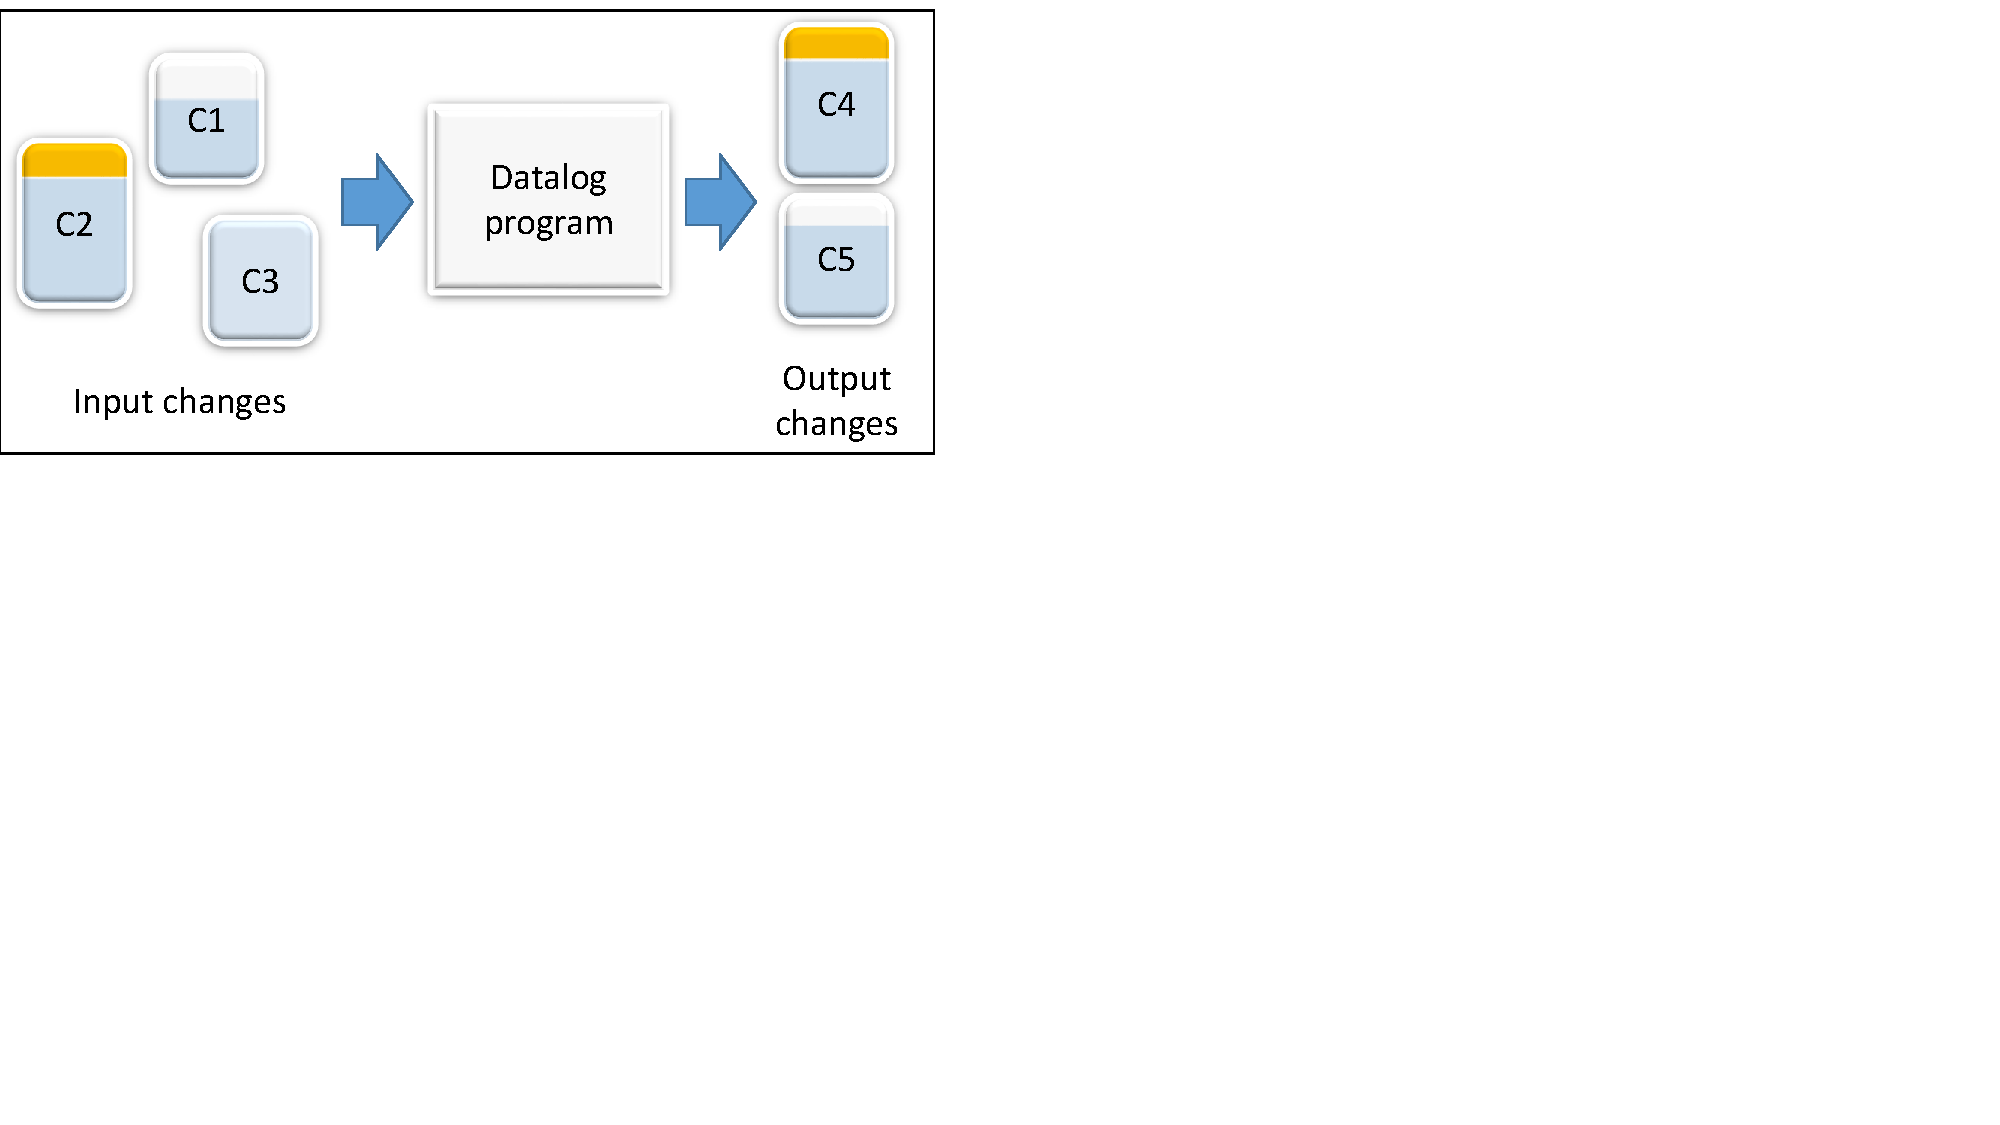
\includegraphics[width=0.5\columnwidth,clip=true,trim=0in 4.4in 6.5in 0in]{differential.pdf}
    \caption{Incremental evaluation of a Datalog program.\label{fig:differential}}
\end{figure}

Here we give a brief overview of the language; the DDlog language
reference~\cite{ddlog-manual} and tutorial~\cite{ddlog-tutorial}
provide a detailed presentation of language features.

\subsection{Type system.}

DDlog is a statically-checked, strongly-typed language; users specify
types for relations, variables, functions, but often DDlog can infer
types from the context.  The type system is inspired by Haskell, and
supports a rich set of types.  Base types include Booleans,
bit-strings (e.g., \texttt{bit<32>}), infinite-precision integers
(\texttt{bigint}), and UTF-8 strings.  Derived types are tuples,
structures, and tagged unions (which generalize enumerated types).  We
currently do not allow defining recursive types like lists or trees; however
DDlog contains three built-in collection types: maps, sets, and arrays
(described in Section~\ref{sec:collections}).  Figure~\ref{fig:types}
shows several type declarations.

Generic types are supported; type variables are syntactically
distinguished by a tick: \texttt{'A}.  The language
contains a built-in reference type \texttt{Ref<'T>}.  Unlike other
languages, two references are equal if the objects referred are equal;
thus references do not alter the nature of Datalog.  References can be
used to reduce memory consumption when complex objects are stored in
multiple relations.

\begin{figure}[t]
  \footnotesize
\begin{lstlisting}[language=ddlog]
// A tagged-union type
typedef IPAddress = IPv4Address{ipv4addr: bit<32>}
                  | IPv6Address{ipv6addr: bit<128>}
// A generic option type
typedef Option<'A> = None
                   | Some{value: 'A}
typedef OptionalIPAddress = Option<IPAddress>
\end{lstlisting}
\caption{Type declarations in DDlog.  \texttt{None}, \texttt{Some},
\texttt{IPv6Address} are \emph{pattern constructors}.\label{fig:types}}
\end{figure}

\subsection{Relations and Rules.}

Relations are strongly typed; the value in each column must have a
statically-determined type.  There are three kinds of relations in
DDlog:

\noindent \textbf{Input relations:} the content of these relations is provided by
the environment, in an incremental way.

\noindent \textbf{Output relations:} these are computed by the DDlog
program, and the DDlog runtime will inform the environment of changes
in these relations.

\noindent \textbf{Intermediate relations:} these are also computed by
the DDlog program, but they are hidden from the environment.

Figure~\ref{fig:relations-rules} shows three relation declarations.
An input relation may declare an optional primary key --- which is a
set of columns that can be used to delete entries efficiently by
specifying only the key.

\begin{figure}[t]
  \small
  \begin{lstlisting}[language=ddlog]
input relation Edge(from: node_t, to: node_t)
                    primary key (e) e.from
input relation Exclude(node: node_t)
output relation Path(src: node_t, dst: node_t)
/* The Path relation is computed as a union of two rules */
// Rule 1: base case
Path(x, y) :- Edge(x,y).
// Rule 2: recursive step: join Path relation with Edge
// followed by an antijoin with Exclude.
Path(x, z) :- Path(x, w), Edge(w, z), not Exclude(z).
  \end{lstlisting}
  \caption{A graph described by two relations and a rule to compute
    paths in the graph that exclude some nodes.\label{fig:relations-rules}}
\end{figure}

DDlog rules are composed of standard Datalog operators: joins, antijoins, and
unions, illustrated in Figure~\ref{fig:relations-rules}, as
well as aggregation, and flatmap, discussed in Section~\ref{sec:collections}.
DDlog allows recursive rules with stratified negation: intuitively, a DDlog
relation cannot recursively depend on its own negation.

\subsection{Computations in rules.}

Much of DDlog's power stems from its ability to perform complex
computation inside rules.  For example, the rule in
Figure~\ref{fig:area} computes an inner join of height and width
tables on the object id column, and then computes the area of the
object as the product of its height and width.

\begin{figure}[t]
  \footnotesize
  \begin{lstlisting}[language=ddlog]
input relation Height(object_id: int, height: int)
input relation Width(object_id: int, width: int)
output relation Area(object_id: int, area: int)
// Compute the area of an object as the product of
// its height and width.
Area(oid, area) :- Height(oid, h), Width(oid, w),
                   var area = w * h.

// Alternative syntax for defining the same relation.
for o in Height // o is a tuple with fields (object_id, height)
   for o1 in Width if o1.oid == o.oid
       Area(o.oid, o1.width * o.height)
  \end{lstlisting}
  \caption{Rule examples.  The first rule uses expressions and
    variables --- \texttt{var} introduces a \emph{variable binding}.
    The second rule is equivalent with the first one, but is written
    using an imperative-style syntax.\label{fig:area}}
\end{figure}

The DDlog expression language supports arithmetic, string
manipulation, control flow constructs and function calls.

\paragraph{Local variables.}
Local variables are used to store intermediate results of
computations.  In DDlog, local variables can be introduced in three
different contexts: (1) variables can be defined directly in the body
of a rule, e.g., the \texttt{area} variable in Figure~\ref{fig:area};
(2) a variable can be defined in a \texttt{match} pattern, as in
Figure~\ref{fig:function}; and (3) finally, a variable can be defined
inside an expression, e.g., the \texttt{res} variable in
Figure~\ref{fig:collections}.  A variable is visible within the
syntactic scope where it was defined.

\paragraph{``Imperative'' rule syntax.}
We have also defined an alternative syntax for rules, inspired by the
FLWOR syntax of XQuery expressions~\cite{boag-xquery02}.  The
``imperative'' fragment offers several statements: \texttt{skip} (does
nothing), \texttt{for}, \texttt{if}, \texttt{match}, block statements
(enclosed in braces), and variable definitions \texttt{var...in}.  An
example is shown in Figure~\ref{fig:area}.  This language is
essentially a language of monoid
comprehensions~\cite{fegaras-sigmod95}, so it is easily converted to a
traditional Datalog representation using a syntax-directed translation
in the compiler front-end.  Recursive relations cannot be expressed
using this syntax.

\paragraph{Integers.} The integer types (\texttt{bigint} and \texttt{bit<N>}) provide the
standard arithmetic operations, as well as bit-wise operations, bit
selection \texttt{v[15:8]}, shifting, and concatenation.

\paragraph{Strings} All primitive types contain built-in conversions to strings, and users
can implement string conversion functions for user-defined types (like
Java's \texttt{toString()} method).  Expressions enclosed within
\texttt{\$\{...\}} in a string literal are \emph{interpolated}: they
are evaluated at run-time, converted to strings and substituted; this
is a feature inspired by JavaScript; for example
\texttt{"x+y=\$\{x+y\}"}.

\begin{figure}[t]
  \footnotesize
  \begin{lstlisting}[language=ddlog]
function lastByte(a: OptionalIPAddress): bit<8> = {
  match (a) {
    None -> 0,
    Some{IPv4Address{.ipv4addr = addr}} -> addr[7:0],
    Some{IPv6Address{.ipv6addr = addr}} -> addr[7:0]
  }
}
relation Host(address: OptionalIPAddress)
// Rule that performs matching on address structure
IPv6Addr(addr) :- Host(.address=Some{IPv6Address{addr}}).
  \end{lstlisting}
\caption{Pattern matching used in a DDlog function and in a rule.\label{fig:function}}
\end{figure}

\paragraph{Pattern matching.}  DDlog borrows
the \texttt{match} expression from ML and Haskell; a \texttt{match}
expression simultaneously performs pattern-matching against type
constructors or values, and also can bind values.
Figure~\ref{fig:function} shows a \texttt{match} expression that uses
a nested pattern to extract a byte from a value \texttt{a} with type
\texttt{OptionalIPAddress} (this type was defined in
Figure~\ref{fig:types}).  For example, the last case binds the
\texttt{addr} variable to the value of the \texttt{ipv6addr} field.

Pattern matching can also be used directly in the body of a rule, as
in the last line from Figure~\ref{fig:function}, which extracts only
IPv6 addresses from the \texttt{Host} relation and binds their value
to the \texttt{addr} variable, which in turn is used in the left-hand side of
the rule defining \texttt{IPv6Addr} relation.

\paragraph{Functions.}

DDlog functions encapsulate pure (side-effect-free) computations.
Example functions are \texttt{lastByte} from
Figure~\ref{fig:function}, and \texttt{concat} from
Figure~\ref{fig:collections}.  Recursive functions are not supported.
Users and libraries can declare prototypes of \texttt{extern}
functions, which must be implemented outside of DDlog (e.g., in Rust),
and linked against the DDlog program at link time.  The compiler
assumes that extern functions are pure.

\subsection{Collections}\label{sec:collections}

The DDlog standard library contains three built-in generic collection
types (implemented natively in Rust): \texttt{Vec<'T>},
\texttt{Set<'T>} and \texttt{Map<'K, 'V>}.  Values of these types can
be stored as first-class values within relations.  Equality for values
of these types is defined element-wise.  In theory such types are not
necessary, since collections within relations can be represented using
separate relations.  We have introduced them into the language because
many practical applications have data models that contain nested
collections; by supporting collection-valued columns natively in DDlog
we can more easily interface with such applications, without the need
to write glue code to convert collections back and forth into separate
relations using foreign keys.

Figure~\ref{fig:collections} shows the declaration in DDlog of an
external function which splits a string into substrings using a
separator; this function returns a vector of strings.

\begin{figure}[t]
  \footnotesize
  \begin{lstlisting}[language=ddlog]
// declare external function returning a vector of strings
extern function split(s: string, sep: string): Vec<string>
// DDlog function to concatenate all elements of a vector
function concat(s: Vec<string>, sep: string): string = {
  var res = "";
  for (e in s) {
    res = (if (res != "") (res + sep) else res) + e
  };
  res   // last value is function evaluation result
}

input relation Phrases(p: string)
relation Words(w: string)
// Words contains all words that appear in some phrase
Words(w) :- Phrases(p), var w = FlatMap(split(p, " ")).

// Shortest path between each pair of points x, y
// (x, y) is the key for grouping
// min is the function used to aggregate data in each group
ShortestPath(x, y, min_cost) :- Path(x, y, cost),
                 var min_cost = Aggregate((x, y), min(cost)).
\end{lstlisting}
\caption{Operations on collections: iteration, flattening,
  aggregation.\label{fig:collections}}
\end{figure}

\texttt{for} loops can be used to iterate over elements in
collections.  Figure~\ref{fig:collections} shows an implementation of
the function \texttt{concat}, the inverse of \texttt{split}, which
uses a loop.

The \texttt{FlatMap} operator can be used to flatten
a collection into a set of DDlog records, as illustrated in the definition of
relation \texttt{Words} in Figure~\ref{fig:collections}.

The \texttt{Aggregate} operator can be used to evaluate the equivalent
of SQL groupby-aggregate queries.  The aggregate operator has two
arguments: a key function, and an aggregation function.  The
aggregation function receives a group of
records that share the same key.  The
\texttt{ShortestPath} relation in Figure~\ref{fig:collections} is
computed using aggregation.

\subsection{Module system}

DDlog offers a simple module system, inspired by Haskell and Python,
which allows importing definitions (types, functions, relations) from
multiple files.  The user can add imported definitions directly into the
name space of the importing module or keep them in a separate name space to
prevent name collisions.  Similar to Java packages, module names are
hierarchical and the module name hierarchy must match the paths on the
the filesystem where modules are stored.  The directive \texttt{import
  library.module} will load the module from file
\texttt{library/module.dl}.

The DDlog \emph{standard library} is a module containing a growing
collection of useful functions and data structures: some generic
functions and data-types, such as \texttt{min}, string manipulation
and conversion to strings, functions to manipulate vectors, sets, maps
(insertion, deletion, lookup, etc.).

%\subsection{``Imperative'' relation definitions}
